

\tikzset{every picture/.style={line width=0.75pt}} %set default line width to 0.75pt        

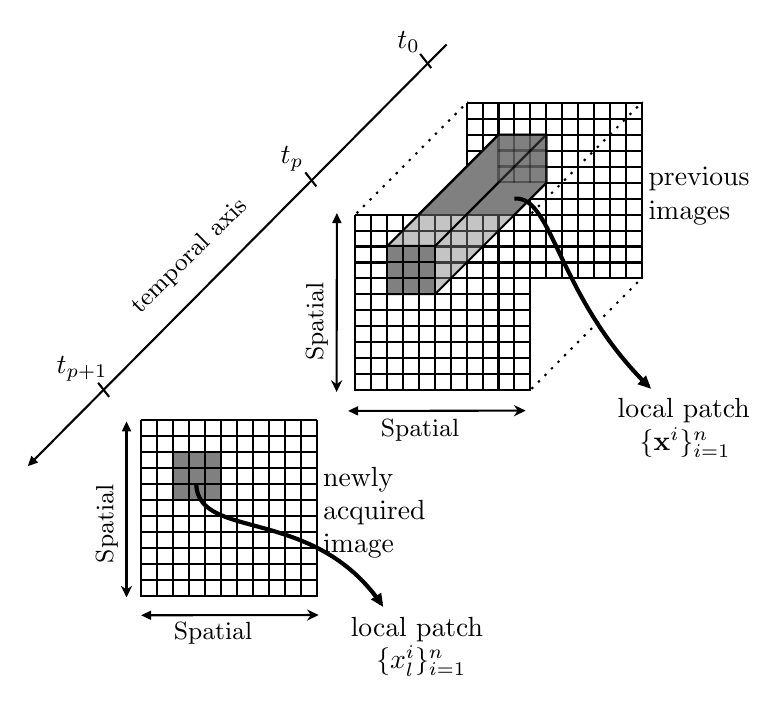
\begin{tikzpicture}[x=0.4pt,y=0.4pt,yscale=-1,xscale=1]
%uncomment if require: \path (0,656); %set diagram left start at 0, and has height of 656



%Shape: Grid [id:dp7338770920799249] 
\draw  [draw opacity=0][fill={rgb, 255:red, 255; green, 255; blue, 255 }  ,fill opacity=1 ] (425.4,79.84) -- (584.33,79.84) -- (584.33,239.31) -- (425.4,239.31) -- cycle ; \draw   (425.4,79.84) -- (425.4,239.31)(439.82,79.84) -- (439.82,239.31)(454.23,79.84) -- (454.23,239.31)(468.65,79.84) -- (468.65,239.31)(483.06,79.84) -- (483.06,239.31)(497.48,79.84) -- (497.48,239.31)(511.89,79.84) -- (511.89,239.31)(526.31,79.84) -- (526.31,239.31)(540.72,79.84) -- (540.72,239.31)(555.14,79.84) -- (555.14,239.31)(569.55,79.84) -- (569.55,239.31)(583.97,79.84) -- (583.97,239.31) ; \draw   (425.4,79.84) -- (584.33,79.84)(425.4,94.25) -- (584.33,94.25)(425.4,108.67) -- (584.33,108.67)(425.4,123.08) -- (584.33,123.08)(425.4,137.5) -- (584.33,137.5)(425.4,151.91) -- (584.33,151.91)(425.4,166.33) -- (584.33,166.33)(425.4,180.74) -- (584.33,180.74)(425.4,195.16) -- (584.33,195.16)(425.4,209.57) -- (584.33,209.57)(425.4,223.99) -- (584.33,223.99)(425.4,238.4) -- (584.33,238.4) ; \draw    ;
%Shape: Cube [id:dp5674870079269827] 
\draw  [fill={rgb, 255:red, 128; green, 128; blue, 128 }  ,fill opacity=1 ] (353.98,208.76) -- (454.31,108.43) -- (497.48,108.43) -- (497.48,151.91) -- (397.15,252.25) -- (353.98,252.25) -- cycle ; \draw   (497.48,108.43) -- (397.15,208.76) -- (353.98,208.76) ; \draw   (397.15,208.76) -- (397.15,252.25) ;
%Shape: Grid [id:dp8494480792086485] 
\draw  [draw opacity=0][fill={rgb, 255:red, 255; green, 255; blue, 255 }  ,fill opacity=1 ][line width=0.75]  (324.5,180.74) -- (483.42,180.74) -- (483.42,340.21) -- (324.5,340.21) -- cycle ; \draw  [line width=0.75]  (324.5,180.74) -- (324.5,340.21)(338.91,180.74) -- (338.91,340.21)(353.33,180.74) -- (353.33,340.21)(367.74,180.74) -- (367.74,340.21)(382.16,180.74) -- (382.16,340.21)(396.57,180.74) -- (396.57,340.21)(410.99,180.74) -- (410.99,340.21)(425.4,180.74) -- (425.4,340.21)(439.82,180.74) -- (439.82,340.21)(454.23,180.74) -- (454.23,340.21)(468.65,180.74) -- (468.65,340.21)(483.06,180.74) -- (483.06,340.21) ; \draw  [line width=0.75]  (324.5,180.74) -- (483.42,180.74)(324.5,195.16) -- (483.42,195.16)(324.5,209.57) -- (483.42,209.57)(324.5,223.99) -- (483.42,223.99)(324.5,238.4) -- (483.42,238.4)(324.5,252.82) -- (483.42,252.82)(324.5,267.23) -- (483.42,267.23)(324.5,281.65) -- (483.42,281.65)(324.5,296.06) -- (483.42,296.06)(324.5,310.48) -- (483.42,310.48)(324.5,324.89) -- (483.42,324.89)(324.5,339.31) -- (483.42,339.31) ; \draw  [line width=0.75]   ;
%Straight Lines [id:da659221038660974] 
\draw  [dash pattern={on 0.84pt off 2.51pt}]  (484.05,338.13) -- (584.58,237.22) ;
%Straight Lines [id:da7683082470179678] 
\draw  [dash pattern={on 0.84pt off 2.51pt}]  (326.08,179.57) -- (426.61,78.66) ;
%Straight Lines [id:da9442765255539709] 
\draw  [dash pattern={on 0.84pt off 2.51pt}]  (484.05,179.57) -- (584.58,78.66) ;
%Shape: Cube [id:dp38890234688871517] 
\draw  [fill={rgb, 255:red, 128; green, 128; blue, 128 }  ,fill opacity=0.46 ] (353.9,209) -- (454.23,108.67) -- (497.4,108.67) -- (497.4,152.15) -- (397.07,252.48) -- (353.9,252.48) -- cycle ; \draw   (497.4,108.67) -- (397.07,209) -- (353.9,209) ; \draw   (397.07,209) -- (397.07,252.48) ;
%Straight Lines [id:da40601813316520086] 
\draw    (308.23,182.4) -- (308,338) ;
\draw [shift={(308,341)}, rotate = 270.08] [fill={rgb, 255:red, 0; green, 0; blue, 0 }  ][line width=0.08]  [draw opacity=0] (10.72,-5.15) -- (0,0) -- (10.72,5.15) -- (7.12,0) -- cycle    ;
\draw [shift={(308.24,179.4)}, rotate = 90.08] [fill={rgb, 255:red, 0; green, 0; blue, 0 }  ][line width=0.08]  [draw opacity=0] (8.93,-4.29) -- (0,0) -- (8.93,4.29) -- cycle    ;
%Straight Lines [id:da8951999998317222] 
\draw    (321.45,358.07) -- (475.76,357.83) ;
\draw [shift={(478.76,357.83)}, rotate = 179.91] [fill={rgb, 255:red, 0; green, 0; blue, 0 }  ][line width=0.08]  [draw opacity=0] (10.72,-5.15) -- (0,0) -- (10.72,5.15) -- (7.12,0) -- cycle    ;
\draw [shift={(318.45,358.07)}, rotate = 359.91] [fill={rgb, 255:red, 0; green, 0; blue, 0 }  ][line width=0.08]  [draw opacity=0] (8.93,-4.29) -- (0,0) -- (8.93,4.29) -- cycle    ;
%Shape: Grid [id:dp3376575506625188] 
\draw  [draw opacity=0][fill={rgb, 255:red, 128; green, 128; blue, 128 }  ,fill opacity=1 ] (353.9,209.24) -- (398.09,209.24) -- (398.09,253.36) -- (353.9,253.36) -- cycle ; \draw   (353.9,209.24) -- (353.9,253.36)(368.32,209.24) -- (368.32,253.36)(382.73,209.24) -- (382.73,253.36)(397.15,209.24) -- (397.15,253.36) ; \draw   (353.9,209.24) -- (398.09,209.24)(353.9,223.65) -- (398.09,223.65)(353.9,238.07) -- (398.09,238.07)(353.9,252.48) -- (398.09,252.48) ; \draw    ;
%Shape: Grid [id:dp5165624876504162] 
\draw  [draw opacity=0][fill={rgb, 255:red, 128; green, 128; blue, 128 }  ,fill opacity=0.27 ] (454.23,108.43) -- (498.42,108.43) -- (498.42,152.55) -- (454.23,152.55) -- cycle ; \draw  [color={rgb, 255:red, 0; green, 0; blue, 0 }  ,draw opacity=0.35 ] (454.23,108.43) -- (454.23,152.55)(468.65,108.43) -- (468.65,152.55)(483.06,108.43) -- (483.06,152.55)(497.48,108.43) -- (497.48,152.55) ; \draw  [color={rgb, 255:red, 0; green, 0; blue, 0 }  ,draw opacity=0.35 ] (454.23,108.43) -- (498.42,108.43)(454.23,122.85) -- (498.42,122.85)(454.23,137.26) -- (498.42,137.26)(454.23,151.68) -- (498.42,151.68) ; \draw  [color={rgb, 255:red, 0; green, 0; blue, 0 }  ,draw opacity=0.35 ]  ;

%Shape: Grid [id:dp1899080303582048] 
\draw  [draw opacity=0][fill={rgb, 255:red, 255; green, 255; blue, 255 }  ,fill opacity=1 ] (131.48,366.33) -- (290.41,366.33) -- (290.41,525.8) -- (131.48,525.8) -- cycle ; \draw   (131.48,366.33) -- (131.48,525.8)(145.9,366.33) -- (145.9,525.8)(160.31,366.33) -- (160.31,525.8)(174.73,366.33) -- (174.73,525.8)(189.14,366.33) -- (189.14,525.8)(203.56,366.33) -- (203.56,525.8)(217.97,366.33) -- (217.97,525.8)(232.39,366.33) -- (232.39,525.8)(246.8,366.33) -- (246.8,525.8)(261.22,366.33) -- (261.22,525.8)(275.63,366.33) -- (275.63,525.8)(290.05,366.33) -- (290.05,525.8) ; \draw   (131.48,366.33) -- (290.41,366.33)(131.48,380.74) -- (290.41,380.74)(131.48,395.16) -- (290.41,395.16)(131.48,409.57) -- (290.41,409.57)(131.48,423.99) -- (290.41,423.99)(131.48,438.4) -- (290.41,438.4)(131.48,452.82) -- (290.41,452.82)(131.48,467.23) -- (290.41,467.23)(131.48,481.65) -- (290.41,481.65)(131.48,496.06) -- (290.41,496.06)(131.48,510.48) -- (290.41,510.48)(131.48,524.89) -- (290.41,524.89) ; \draw    ;
%Straight Lines [id:da4322454502328483] 
\draw    (134.48,542.7) -- (288.8,542.46) ;
\draw [shift={(291.8,542.46)}, rotate = 179.91] [fill={rgb, 255:red, 0; green, 0; blue, 0 }  ][line width=0.08]  [draw opacity=0] (10.72,-5.15) -- (0,0) -- (10.72,5.15) -- (7.12,0) -- cycle    ;
\draw [shift={(131.48,542.7)}, rotate = 359.91] [fill={rgb, 255:red, 0; green, 0; blue, 0 }  ][line width=0.08]  [draw opacity=0] (8.93,-4.29) -- (0,0) -- (8.93,4.29) -- cycle    ;
%Straight Lines [id:da9290493372472008] 
\draw    (118.2,370.6) -- (118.2,523.6) ;
\draw [shift={(118.2,526.6)}, rotate = 270] [fill={rgb, 255:red, 0; green, 0; blue, 0 }  ][line width=0.08]  [draw opacity=0] (10.72,-5.15) -- (0,0) -- (10.72,5.15) -- (7.12,0) -- cycle    ;
\draw [shift={(118.2,367.6)}, rotate = 90] [fill={rgb, 255:red, 0; green, 0; blue, 0 }  ][line width=0.08]  [draw opacity=0] (8.93,-4.29) -- (0,0) -- (8.93,4.29) -- cycle    ;
%Shape: Grid [id:dp046588246064819705] 
\draw  [draw opacity=0][fill={rgb, 255:red, 128; green, 128; blue, 128 }  ,fill opacity=1 ] (160.21,395.16) -- (204.39,395.16) -- (204.39,439.28) -- (160.21,439.28) -- cycle ; \draw   (160.21,395.16) -- (160.21,439.28)(174.62,395.16) -- (174.62,439.28)(189.04,395.16) -- (189.04,439.28)(203.45,395.16) -- (203.45,439.28) ; \draw   (160.21,395.16) -- (204.39,395.16)(160.21,409.57) -- (204.39,409.57)(160.21,423.99) -- (204.39,423.99)(160.21,438.4) -- (204.39,438.4) ; \draw    ;
%Curve Lines [id:da9756715446691779] 
\draw [line width=1.5]    (181.16,424.4) .. controls (183.25,475.65) and (287.01,443.2) .. (348.16,532.26) ;
\draw [shift={(350,535)}, rotate = 236.64] [fill={rgb, 255:red, 0; green, 0; blue, 0 }  ][line width=0.08]  [draw opacity=0] (11.61,-5.58) -- (0,0) -- (11.61,5.58) -- cycle    ;
%Straight Lines [id:da9112439822708085] 
\draw    (31.11,405.87) -- (407.3,27.1) ;
\draw [shift={(29,408)}, rotate = 314.8] [fill={rgb, 255:red, 0; green, 0; blue, 0 }  ][line width=0.08]  [draw opacity=0] (8.93,-4.29) -- (0,0) -- (8.93,4.29) -- cycle    ;
%Straight Lines [id:da33689275765049076] 
\draw    (279.73,142.61) -- (289.67,155.31) ;
%Straight Lines [id:da5111940194111664] 
\draw    (383.47,35.59) -- (393.41,48.3) ;
%Straight Lines [id:da029907205732478515] 
\draw    (92.55,332.67) -- (102.49,345.38) ;
%Curve Lines [id:da7608806482218253] 
\draw [line width=1.5]    (468.65,166.33) .. controls (503.14,162.96) and (507.43,255.2) .. (589.49,335.57) ;
\draw [shift={(592,338)}, rotate = 223.77] [fill={rgb, 255:red, 0; green, 0; blue, 0 }  ][line width=0.08]  [draw opacity=0] (11.61,-5.58) -- (0,0) -- (11.61,5.58) -- cycle    ;

% Text Node
\draw (399.65,375.3) node  [font=\small] [align=left] {\begin{minipage}[lt]{41.32pt}\setlength\topsep{0pt}
Spatial
\end{minipage}};
% Text Node
\draw (290.44,255.23) node  [font=\small,rotate=-270.23] [align=left] {\begin{minipage}[lt]{46.1pt}\setlength\topsep{0pt}
Spatial
\end{minipage}};
% Text Node
\draw (586.97,135.25) node [anchor=north west][inner sep=0.75pt]   [align=left] {previous\\images};
% Text Node
\draw (52.35,305.64) node [anchor=north west][inner sep=0.75pt]    {$t_{p+1}$};
% Text Node
\draw (202.78,207.15) node  [font=\small,rotate=-315.27,xslant=0] [align=left] {\begin{minipage}[lt]{77.06pt}\setlength\topsep{0pt}
temporal axis\\
\end{minipage}};
% Text Node
\draw (360.1,12.8) node [anchor=north west][inner sep=0.75pt]    {$t_{0}$};
% Text Node
\draw (254.57,116.38) node [anchor=north west][inner sep=0.75pt]    {$t_{p}$};
% Text Node
\draw (579,370.4) node [anchor=north west][inner sep=0.75pt]    {$\{\mathbf{x}^{i} \}_{i=1}^{n}$};
% Text Node
\draw (559,344) node [anchor=north west][inner sep=0.75pt]   [align=left] {local patch};
% Text Node
\draw (212.68,558.94) node  [font=\small] [align=left] {\begin{minipage}[lt]{41.32pt}\setlength\topsep{0pt}
Spatial
\end{minipage}};
% Text Node
\draw (100.73,443.7) node  [font=\small,rotate=-270.23] [align=left] {\begin{minipage}[lt]{41.47pt}\setlength\topsep{0pt}
Spatial
\end{minipage}};
% Text Node
\draw (293.05,405.89) node [anchor=north west][inner sep=0.75pt]   [align=left] {newly \\acquired \\image};
% Text Node
\draw (341,567.4) node [anchor=north west][inner sep=0.75pt]    {$\{x_{l}^{i} \}_{i=1}^{n}$};
% Text Node
\draw (318,542) node [anchor=north west][inner sep=0.75pt]   [align=left] {local patch};


\end{tikzpicture}
